\documentclass[a4paper,11pt]{article}
\usepackage[polish]{babel}
\usepackage[OT4]{fontenc}
\usepackage[utf8]{inputenc}
\usepackage{graphicx}
\usepackage{subfig}
\usepackage{epstopdf}




\date{16/03/2014}


%opening
\title{PAMSI -- testowanie implementacji struktur danych}
\author{Piotr Wilkosz}
\captionsetup{belowskip=12pt,aboveskip=4pt}
\begin{document}

\maketitle

\section{Wstęp}
Celem ćwiczenia było przetestowanie implementacji takich struktur danych jak:
  \begin{itemize}
   \item Stos --- zawierający listę lub tablicę dynamiczną
   \item Kolejka --- zawierająca listę lub tablicę dynamiczną
  \end{itemize}
Zadaniem było zmierzenie czasu wykonywania operacji wypełnienia powyższych struktor danych.
\section{Wyniki pomiarów}
\begin{enumerate}
 \item Stos bazujący na liście:
   
  \begin{table}[th]
  \centering
    \caption{Pomiar czasu zapełnienia stosu bazującego na liście}

      \begin{tabular}{|l|l|l|}
      
	\hline
	N & czas & odchylenie \\
    \hline
  10 & 3.1777e-06 & 9.66352e-07\\
  \hline
100 & 1.41498e-05 & 1.37796e-06\\
\hline
1000 & 0.000129143 & 1.37132e-05\\
\hline
10000 & 0.00125259 & 0.000136966\\
\hline
50000 & 0.00610872 & 0.000647302\\
\hline
100000 & 0.0148653 & 0.00293036\\
\hline
    \end{tabular}
    \end{table}
    \newpage
 \begin{figure}[th]
\centering
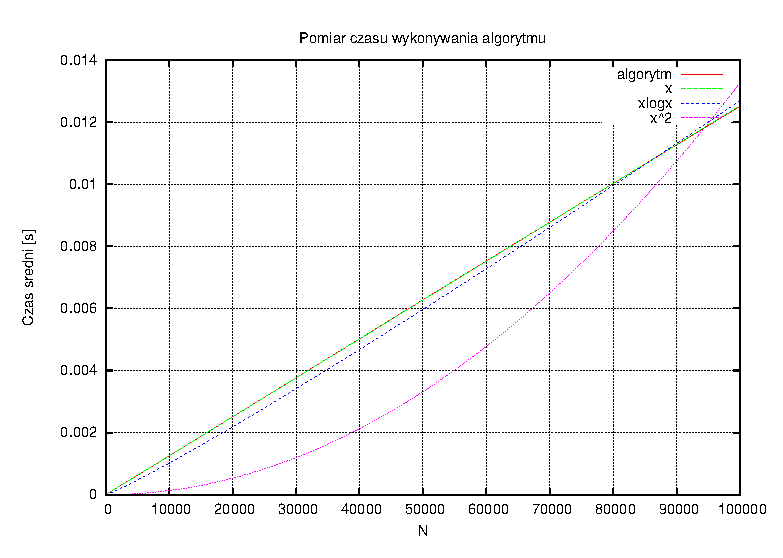
\includegraphics[width=0.8\textwidth]{wykres1.eps}
\caption{Wykres do tabeli 1}
\label{Wykres do tabeli 1}
\end{figure} 
Na podstawie wykresu złożoność obliczeniową algorytmu zapełnienia stosu bazującego na liście szacuje się na $ O(n) $.

\item Stos bazujący na tablicy dynamicznej, każdorazowo powiększającej swój rozmiar:

  \begin{table}[th]
  \centering
    \caption{Pomiar czasu zapełnienia stosu bazującego na tablicy dynamicznej; każdorazowe powiększanie pamięci}

      \begin{tabular}{|l|l|l|}
	\hline
	N & czas & odchylenie\\
    \hline
    10 & 5.2315e-06 & 1.84447e-06\\
    \hline
100 & 9.61087e-05 & 1.17477e-05\\
\hline
1000 & 0.00626336 & 0.000569029\\
\hline
10000 & 0.602328 & 0.0547606\\
\hline
50000 & 16.1983 & 1.47384\\
\hline
100000 & 63.4257 & 6.11571\\
\hline
    \end{tabular}
    \end{table}
    \newpage
\begin{figure}[th]
\centering
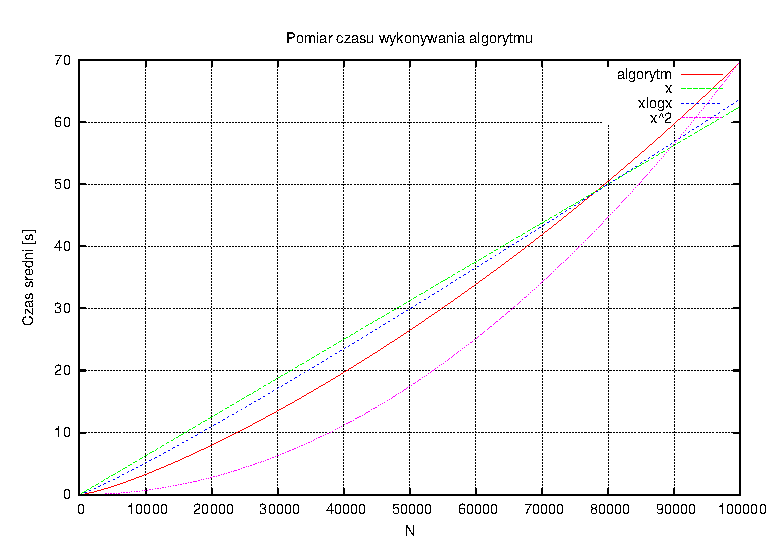
\includegraphics[width=0.8\textwidth]{wykres2.eps}
\caption{Wykres do tabeli 2}
\label{Wykres do tabeli 2}
\end{figure} 

Na podstawie wykresu złożoność obliczeniową algorytmu zapełnienia stosu bazującego na tablicy każdorazowo powiększającej swój rozmiar szacuje się na $ O(n^{2}) $.
\item Stos bazujący na tablicy podwajającej swój rozmiar po zapełnieniu stosu:

\begin{table}[th]
\centering
    \caption{Pomiar czasu zapełnenia stosu bazującego na tablicy; podwajanie pamięci}

      \begin{tabular}{|l|l|l|}
	\hline
	N & czas & odchylenie \\
    \hline
    10 & 2.9054e-06 & 4.54692e-07\\
    \hline
100 & 7.941e-06 & 7.84532e-07\\
\hline
1000& 3.41665e-05 & 3.28946e-06\\
\hline
10000 & 0.000393291 & 4.00849e-05\\
\hline
50000 & 0.0017202 & 0.000172796\\
\hline
100000 & 0.00372878 & 0.00034095\\
\hline
    \end{tabular}
    \end{table}
    \newpage
\begin{figure}[th]
\centering
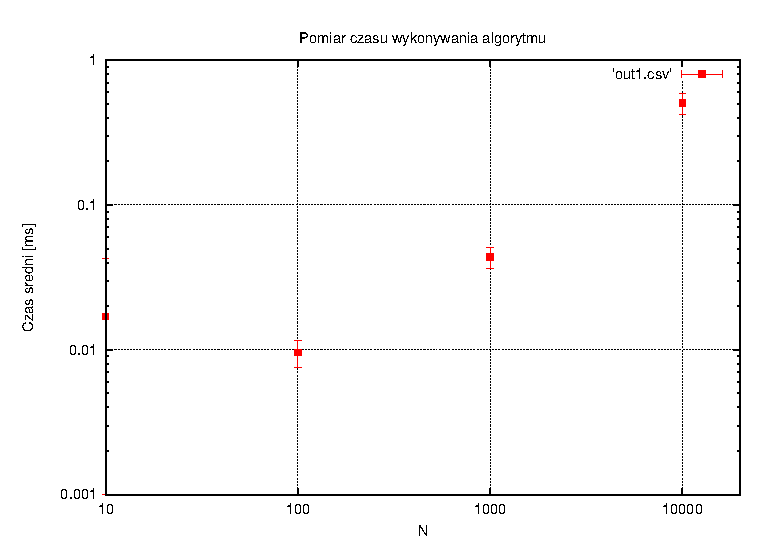
\includegraphics[width=0.8\textwidth]{wykres3.eps}
\caption{Wykres do tabeli 3}
\label{Wykres do tabeli 3}
\end{figure} 

Na podstawie wykresu złożoność obliczeniową algorytmu zapełnienia stosu bazującego na tablicy podwajającej swój rozmiar szacuje się na $ O(n) $.
\item Kolejka bazująca na liście:

\begin{table}[th]
\centering
    \caption{Pomiar zapełnienia koljeki bazującej na liście}

      \begin{tabular}{|l|l|l|}
	\hline
	N & czas & odchylenie \\
    \hline
   10 & 2.9402e-06 & 4.02804e-07\\
   \hline
100 & 1.43175e-05 & 1.45537e-06\\
\hline
1000 & 0.000123787 & 1.32083e-05\\
\hline
10000 & 0.00121058 & 0.000122136\\
\hline
50000 & 0.0060172 & 0.000595832\\
\hline
100000 & 0.012138 & 0.00127857\\
\hline
    \end{tabular}
    \end{table}

\newpage
\begin{figure}[th]
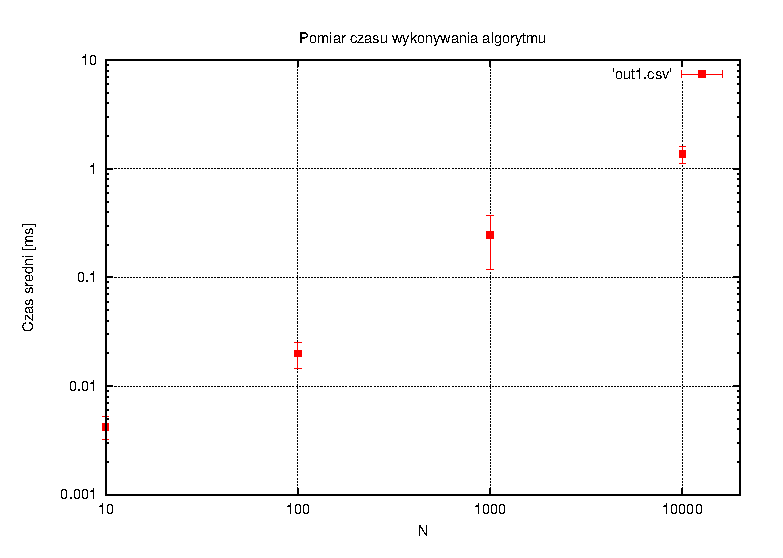
\includegraphics[width=0.8\textwidth]{wykres4.eps}
\caption{Wykres do tabeli 4}
\label{Wykres do tabeli 4}
\end{figure}
Na podstawie wykresu złożoność obliczeniową algorytmu zapełnienia kolejki bazującej na liście szacuje się na $ O(n) $.
\item Kolejka bazująca na tablicy każdorazowo powiększającej swój rozmiar:

\begin{table}[th]
\centering
    \caption{Pomiar czasu zapełnienia kolejki bazującej na tablicy; każdorazowe powiększanie pamięci}

      \begin{tabular}{|l|l|l|}
	\hline
	N & czas & Odchylenie\\
    \hline
    10 & 4.4419e-06 & 1.43333e-06\\
    \hline
100 & 9.5843e-05 & 8.89311e-06\\
\hline
1000 & 0.00578163 & 0.000530114\\
\hline
10000 & 0.56162 & 0.0531706\\
\hline
50000 & 15.1532 & 1.37704\\
\hline
100000 & 57.5228 & 5.79702\\
\hline
    \end{tabular}
    \end{table}
\newpage
\begin{figure}[th]
\centering
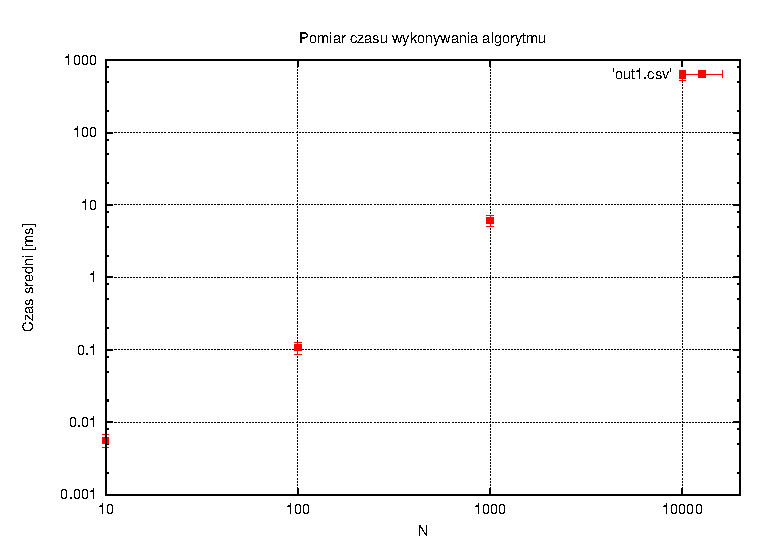
\includegraphics[width=0.8\textwidth]{wykres5.eps}
\caption{Wykres do tabeli 5}
\label{Wykres do tabeli 5}
\end{figure} 
Na podstawie wykresu złożoność obliczeniową algorytmu zapełnienia kolejki bazującej na tablicy każdorazowo powiększającej swój rozmiar szacuje się na $ O(n^{2}) $.
\item Kolejka bazująca na tablicy podwajającej swój rozmiar po zapełnieniu kolejki:

\begin{table}[th]
\centering
    \caption{Pomiar czasu zapełnienia kolejki bazującej na tablicy; podwajanie pamięci}

      \begin{tabular}{|l|l|l|}
	\hline
	N & czas & Odchylenie\\
    \hline
    10 & 2.7934e-06 & 5.70677e-07\\
    \hline
100 & 6.977e-06 & 7.54621e-07\\
\hline
1000 & 3.06953e-05 & 4.08372e-06\\
\hline
10000 & 0.000342118 & 3.42047e-05\\
\hline
50000 & 0.00149814 & 0.000148217\\
\hline
100000 & 0.00326706 & 0.000321491\\

\hline
    \end{tabular}
    \end{table}
    \newpage
\begin{figure}[th]
\centering
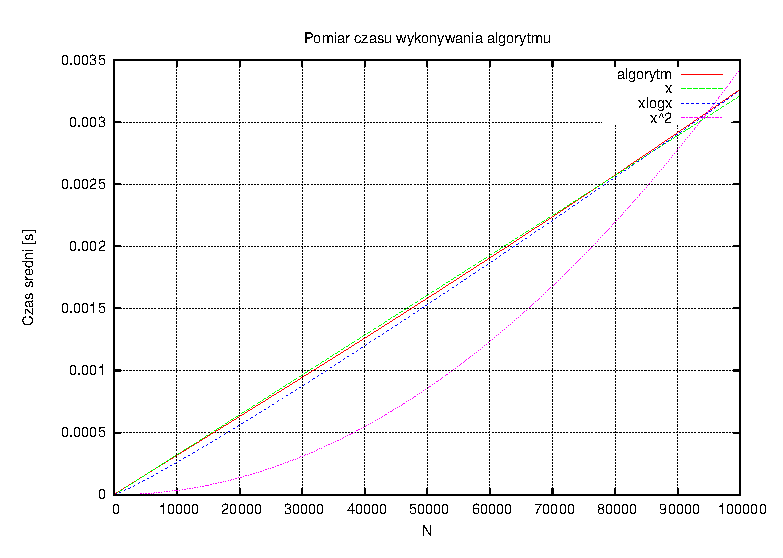
\includegraphics[width=0.8\textwidth]{wykres6.eps}
\caption{Wykres do tabeli 6}
\label{Wykres do tabeli 6}
\end{figure} 
Na podstawie wykresu złożoność obliczeniową algorytmu zapełnienia kolejki bazującej na tablicy podwajającej swój rozmiar szacuje się na $ O(n) $.
\end{enumerate}

\section{Wnioski}

\begin{itemize}
\item Najbardziej wydajne pod względem szybkości wykonania okazały się struktury wykorzystujące listę lub tablicę podwajającą swój rozmiar pod wypełnieniu struktury
Złożoność obliczeniową takiej implementacji szacuje się na $ O(n) $
\item Struktury, które każdorazowo zwiększały rozmiar tablicy działają dużo wolniej, aczkolwiek są oszczędniejsze pod względem zagospodarowania pamięci.
Ich złozoność obliczeniową szacuje się na $ O(n^{2}) $
\end{itemize}
\end{document}
